 
	
		Given equation 
		\begin{align} \label{eq:solutions/1/18/eq:fact1}
			y = x^2-2x+7
		\end{align}
	
		The equation \eqref{eq:solutions/1/18/eq:fact1} can be written as,
		\begin{align}
			x^2-2x-y+7 = 0
		\end{align}
		Comparing it with standard equation,
		\begin{align}
			ax^2+2bxy+cy^2+2dx+2ey+f = 0
		\end{align}
		$\therefore$ a = 1, b = 0, c = 0, d = -1, e = $\frac{-1}{2}$, f = 7.
		\begin{align}
			\therefore \vec{V} = \myvec{a&b\\b&c} = \myvec{1&0\\0&0}
		\end{align} 
		\begin{align}
			\therefore\vec{u} = \myvec{d\\e} = \myvec{-1\\\frac{-1}{2}}\label{eq:solutions/1/18/eq:eq1}
		\end{align}
		\begin{align}
			\mbox{ Now,} \mydet{V} = \mydet{1&0\\0&0} = 0
		\end{align}
		$\implies$ that the curve is a parabola. Now, finding the eigen values corresponding to the $\vec{V}$,
		\begin{align}
			\mydet{\vec{V}-\lambda\vec{I}} = 0
		\end{align}
		\begin{align}
			\mydet{1-\lambda&0\\0&-\lambda} = 0
		\end{align}
		\begin{align}
			\implies \lambda = 0,1.
		\end{align}
		Calculating the eigenvectors corresponding to $\lambda = 0,1$ respectively,
		\begin{align}
			\vec{V}\vec{x} = \lambda\vec{x}
		\end{align}
		\begin{align}
			\myvec{1&0\\0&0}\vec{x} = 0 \implies \vec{p_1} = \myvec{0\\1}
		\end{align}
		\begin{align}
			\myvec{0&0\\0&-1}\vec{x} = \vec{x} \implies \vec{p_2} = \myvec{1\\0}
		\end{align}
		Now by eigen decomposition on $\vec{V}$,
		\begin{align}
			\vec{V} = \vec{PDP^T}
			\label{eq:solutions/1/18/eq:eq2}
		\end{align}
		\begin{align}
			\mbox{where,} \vec{P} = \myvec{\vec{p_1} \vec{p_2}} = \myvec{0&1\\1&0}
		\end{align}
		\begin{align}
			\vec{D} = \myvec{\lambda_1&0\\0&\lambda_2} = \myvec{0&0\\0&1}
		\end{align}
		Hence equation \eqref{eq:solutions/1/18/eq:eq1} becomes,
		\begin{align}
			\vec{V} = \myvec{0&1\\1&0}\myvec{0&0\\0&1}\myvec{0&1\\1&0}
		\end{align}
		\begin{align}
			\vec{V} = \myvec{1&0\\0&0}
		\end{align}
	
	\begin{enumerate}
		\item
							The given parallel line equation is
		\begin{align} 
			\myvec{2 & -1}\vec{x}= -9 \\
			\implies 2x - y + 9 = 0 \label{eq:solutions/1/18/eq:fact2}
		\end{align}
		Now the tangent to parabola is parallel to the line equation \eqref{eq:solutions/1/18/eq:fact2}, the general straight line equation is of the form
		\begin{align}
			ax + by + c = 0
		\end{align}
		The normal vector ($\vec{n}$) and direction ($\vec{m}$) are given by,
		\begin{align} 
			\vec{n} = \myvec{a\\b} \label{eq:solutions/1/18/eq:eq3}\\
			\vec{m} = \myvec{b\\-a} \label{eq:solutions/1/18/eq:eq4}
		\end{align}
		Comparing \eqref{eq:solutions/1/18/eq:fact2}, \eqref{eq:solutions/1/18/eq:eq2}, \eqref{eq:solutions/1/18/eq:eq3}, the direction vectors ($\vec{m}$) and normal ($\vec{n}$)  vectors are,
		\begin{align}
			\vec{m} = \myvec{-1\\-2}\\
			\vec{n} = \myvec{2\\-1}\label{eq:solutions/1/18/eq:eq5}
		\end{align} 
		Now, the equation for the point of contact for the parabola is given as,
		\begin{align}
			\myvec{\vec{u}^T+\kappa\vec{n}^T\\\vec{V}}\vec{q} = \myvec{-f\\\kappa\vec{n}-\vec{u}}\label{eq:solutions/1/18/eq:eq6}\\
			\mbox{where, } \kappa = \frac{\vec{p_1}^T\vec{u}}{\vec{p_1}^T\vec{n}} = \frac{1}{2} \label{eq:solutions/1/18/eq:eq7}
		\end{align}
		Hence substituting the values of \eqref{eq:solutions/1/18/eq:eq1}, \eqref{eq:solutions/1/18/eq:eq5}, \eqref{eq:solutions/1/18/eq:eq2}, \eqref{eq:solutions/1/18/eq:eq7} in equation \eqref{eq:solutions/1/18/eq:eq6} we get,
		\begin{align}
			\myvec{0&-1\\1&0\\0&0}\vec{q} = \myvec{-7\\2\\0}
			\label{eq:solutions/1/18/eq:eq8}
		\end{align}
		Solving for $\vec{q}$ by removing the zero row and representing \eqref{eq:solutions/1/18/eq:eq8} as augmented matrix and then converting the matrix to echelon form,
		\begin{align}
			\implies \myvec{0&-1&-7\\1&0&2} \xleftrightarrow[]{R_1\xleftrightarrow[]{}R_2} \myvec{1&0&2\\0&-1&-7}
		\end{align}
		\begin{align}
			\xleftrightarrow[]{R_2\leftarrow  -R_2} \myvec{1&0&2\\0&1&7}
			\label{eq:solutions/1/18/eq:eq9}
		\end{align}
		Hence from equation \eqref{eq:solutions/1/18/eq:eq9} it can be concluded that the point of contact is,
		\begin{align}
			\vec{q} = \myvec{2\\7}
		\end{align}
		Now $\vec{q}$ is a point on the tangent. Hence, the equation of the
		line can be expressed as
		\begin{align}
			\vec{n}^T\vec{x} = c
			\label{eq:solutions/1/18/eq:eq10}
		\end{align}
		where c is,
		\begin{align}
			c = \vec{n}^T\vec{q} = \myvec{2&-1}\myvec{2\\7} = -3 
			\label{eq:solutions/1/18/eq:eq11}
		\end{align}
		Hence equation of tangent to the curve \eqref{eq:solutions/1/18/eq:fact1} parallel to \eqref{eq:solutions/1/18/eq:fact2} is given by substituting the value of c and $\vec{n}$ from equation \eqref{eq:solutions/1/18/eq:eq11} and \eqref{eq:solutions/1/18/eq:eq5} respectively to the equation \eqref{eq:solutions/1/18/eq:eq10},
		\begin{align}
			\implies\myvec{2&-1}\vec{x} = -3 
		\end{align}
		Figure \ref{eq:solutions/1/18/eq:fig1} verifies that the $\myvec{2&-1}\vec{x} = -3$ is a tangent to parabola  $y = x^2-2x+7$ \\\\
	
	\item
						The given perpendicular line equation is
	\begin{align} 
		\myvec{-15 & 5}\vec{x}= 13 \\
		\implies -15x + 5y - 13 = 0 \label{eq:solutions/1/18/eq:fact3}
	\end{align}
	Now the tangent to parabola is perpendicular to the line equation \eqref{eq:solutions/1/18/eq:fact3}, the general straight line equation is of the form
	\begin{align}
		ax + by + c = 0
	\end{align}
	Therefore, if we find the line that is parallel to the line \eqref{eq:solutions/1/18/eq:fact3}, it will be parallel to the tangent itself. For the given line the normal vector ($\vec{n}$) and direction ($\vec{m}$) are given by,
	\begin{align} 
		\vec{n} = \myvec{a\\b} \label{eq:solutions/1/18/eq:eq12}\\
		\vec{m} = \myvec{b\\-a} \label{eq:solutions/1/18/eq:eq13}
	\end{align}
	Comparing \eqref{eq:solutions/1/18/eq:fact3}, \eqref{eq:solutions/1/18/eq:eq12}, \eqref{eq:solutions/1/18/eq:eq13}, the direction vectors ($\vec{m}$) and normal ($\vec{n}$)  vectors are,
	\begin{align}
		\vec{m} = \myvec{5\\15}\\
		\vec{n} = \myvec{-15\\5}\label{eq:solutions/1/18/eq:eq14}
	\end{align} 

	The parallel line for this vector will have the normal vector ($\vec{n_1}$) and direction ($\vec{m_1}$) are given by
	
		\begin{align}
		\vec{m_1} = \myvec{15\\-5}\\
		\vec{n_1} = \myvec{5\\15}\label{eq:solutions/1/18/eq:eq15}
	\end{align} 
	
	Now, the equation for the point of contact for the parabola is given as,
	\begin{align}
		\myvec{\vec{u}^T+\kappa\vec{n_1}^T\\\vec{V}}\vec{q} = \myvec{-f\\\kappa\vec{n_1}-\vec{u}}\label{eq:solutions/1/18/eq:eq16}\\
		\mbox{where, } \kappa = \frac{\vec{p_1}^T\vec{u}}{\vec{p_1}^T\vec{n_1}} = \frac{-1}{30} \label{eq:solutions/1/18/eq:eq17}
	\end{align}
	Hence substituting the values of \eqref{eq:solutions/1/18/eq:eq1}, \eqref{eq:solutions/1/18/eq:eq15}, \eqref{eq:solutions/1/18/eq:eq2}, \eqref{eq:solutions/1/18/eq:eq17} in equation \eqref{eq:solutions/1/18/eq:eq16} we get,
	\begin{align}
		\myvec{\frac{-7}{6}&-1\\1&0\\0&0}\vec{q} = \myvec{-7\\\frac{5}{6}\\0}
		\label{eq:solutions/1/18/eq:eq18}
	\end{align}
	Solving for $\vec{q}$ by removing the zero row and representing \eqref{eq:solutions/1/18/eq:eq18} as augmented matrix and then converting the matrix to echelon form,
	\begin{align}
		\implies \myvec{\frac{-7}{6}&-1&-7\\1&0&\frac{5}{6}} \xleftrightarrow[]{R_1\xleftrightarrow[]{}R_2} \myvec{1&0&\frac{5}{6}\\\frac{-7}{6}&-1&-7}
	\end{align}
	\begin{align}
		\xleftrightarrow[]{R_2\leftarrow R_2-\brak{\frac{7}{6}}R_1} \myvec{1&0&\frac{5}{6}\\0&-1&\frac{-217}{36}} \\
		\xleftrightarrow[]{R_2\leftarrow  -R_2} \myvec{1&0&\frac{5}{6}\\0&1&\frac{217}{36}}
		\label{eq:solutions/1/18/eq:eq19}
	\end{align}
	Hence from equation \eqref{eq:solutions/1/18/eq:eq19} it can be concluded that the point of contact is,
	\begin{align}
		\vec{q} = \myvec{\frac{5}{6}\\\frac{217}{36}}
	\end{align}
	Now $\vec{q}$ is a point on the tangent. Hence, the equation of the
	line can be expressed as
	\begin{align}
		\vec{n_1}^T\vec{x} = c
		\label{eq:solutions/1/18/eq:eq20}
	\end{align}
	where c is,
	\begin{align}
		c = \vec{n_1}^T\vec{q} = \myvec{5&15}\myvec{\frac{5}{6}\\\frac{217}{36}} = \frac{3405}{36} 
		\label{eq:solutions/1/18/eq:eq21}
	\end{align}
	Hence equation of tangent to the curve \eqref{eq:solutions/1/18/eq:fact1} parallel to \eqref{eq:solutions/1/18/eq:fact3} is given by substituting the value of c and $\vec{n_1}$ from equation \eqref{eq:solutions/1/18/eq:eq21} and \eqref{eq:solutions/1/18/eq:eq15} respectively to the equation \eqref{eq:solutions/1/18/eq:eq20},
	\begin{align}
		\implies\myvec{5&15}\vec{x} = \frac{3405}{36} 
	\end{align}
	Figure \ref{eq:solutions/1/18/eq:fig1} verifies that the $\myvec{5&15}\vec{x} = \frac{3405}{36}$ is a tangent to parabola  $y = x^2-2x+7$
	\begin{figure}
		\centering
		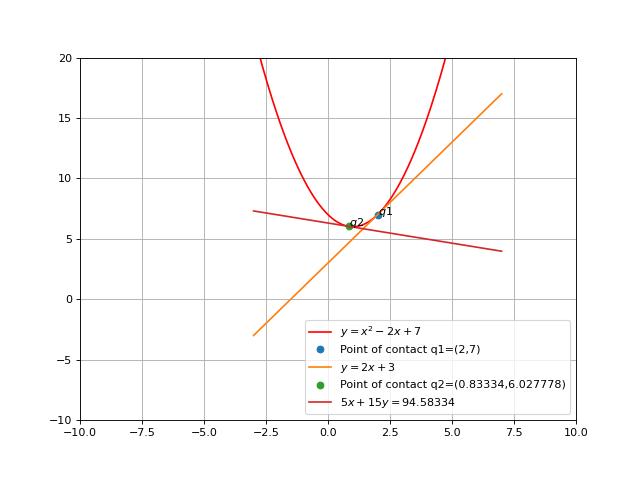
\includegraphics[width=\columnwidth]{./solutions/1/18/codes/parallelPerpendicularLineTangent.png}
		\caption{Tangents to parabola $y = x^2-2x+7$}
		\label{eq:solutions/1/18/eq:fig1}
	\end{figure}

	\end{enumerate}
		
	
